% !TeX root = ../tesis.tex

The commercial software COMSOL Multiphysics™ Ver. 5.4 (COMSOL) allows the user to set a desired geometry for solving Eqs. \eqref{eq:Scatt-Weak-All} as well as the physical properties of each component of the geometry including boundary conditions and the discretization of the system into finite elements.  Additionally, once the Eqs. \eqref{eq:Scatt-Weak-All} are solved, the returned value of the FEM simulation is the total electric field that can be decomposed into an external electric field\footnote{COMSOL's name for the external electric field is the \textit{background electric field}.} $\vb{E}^\text{ext}$, which illuminates the system, and the induced electric field\footnote{COMSOL's name for the induced electric field is the \textit{relative electric field}.} $\vb{E}^\text{ind}$, which corresponds to the scattered (internal) electric field if it is evaluated outside (inside) the scatterer. In this Section a brief summary of the implementation of the scattering  problem with a planar interface and a spherical scatterer is described for users familiarized with the COMSOL interface, where the desired geometry is the setup presented in Fig. \ref{fig:setup} in Section \ref{sec:FEM-Mie} and the external electric field is an incident electric plane wave and a reflected electric plane wave in the upper half volume of the system and a transmitted electric plane wave in the lower half volume of the system. In order to set up the geometry of the system, the boundary conditions and the physical properties of the system, COMSOL's  \textit{Model Builder}  is used.

COMSOL's Model Builder is the internal tool where the user sets all the parameters for the FEM simulation and it is divided into four categories:  Global Definitions, Components, Study and Results. COMSOL allows for several Components and Studies, since they define the Partial Different Equations (PDE) problem to solve, as well as the desired geometry and  physical properties of the system. To build the whole system, geometry and physical properties, one must define the general parameters, then the geometry of the system, afterwards the definition of local variables and operators, later the formulation of the PDE and the external electric field,  then the boundary conditions and, lastly, the meshing of the system.

The Global Definitions allocate the common parameters of any simulation to be performed with its numerical value. Table \ref{tab:Global-parameters} shows the parameters to solve Eq. \eqref{eq:Scatt-Weak-All} considering a spherical scatterer embedded in a matrix conformed by two semiinfinite non-absorbing media forming a planar interface between them. The parameters in Table \ref{tab:Global-parameters} include the properties of the incident electric plane wave ---its amplitude (\lstinline!E_0!),  wavelength (\lstinline!wlength!), traveling direction (\lstinline!theta_i! and \lstinline!phi!) and its polarization through \lstinline!alpha!, a parameters which is $0^\circ$ for \textit{s} polarization and $90^\circ$ for \textit{p} polarization---, the physical properties of the spherical scatterer such as its radius  (\lstinline!radius_NP!) and position in the $z$-plane (\lstinline!h_center!), and the physical properties of the matrices ---the refractive indices of the incidence (\lstinline!n_i!) and transmission (\lstinline!n_t!) media and its width (\lstinline!d_matrix!)---.

\begin{table}[t!]
 \caption{Global definitions for COMSOL simulation: Parameters }
 \label{tab:Global-parameters}
 \centering
 \small
    \begin{tabular}{ |l|l|l| }
     \hline
     \textbf{Name}          &   \textbf{Expression}                              &   \textbf{Description} \\ \hline \hline
     \lstinline!E_0!        &   \lstinline!1. [V/m]!                             &   Incident electric field amplitude \\
     \lstinline!wlength!    &   \lstinline!550. [nm]!                            &   Wavelength of incident plane wave \\
     \lstinline!theta_i!    &   \lstinline!0. [deg]!                             &   (Polar) angle of incidence \\
     \lstinline!phi!        &   \lstinline!0. [deg]!                             &   (Azimuthal) angle of incidence \\
     \lstinline!alpha!      &   \lstinline!0. [deg]!                             &   Electric field inclination \\
     \lstinline!E_s!        &   \lstinline!E_0 * cos(alpha)!                     &   Electric field amplitude (\textit{s} pol) \\
     \lstinline!E_p!        &   \lstinline!E_0 * sin(alpha)!                     &   Electric field amplitude \textit{p} pol) \\
     \lstinline!n_i!        &   \lstinline!1.0!                                  &   Refractive index of the incidence side \\
     \lstinline!n_t!        &   \lstinline!1.5!                                  &   Refractive index of the transmssion side \\
     \lstinline!radius_NP!  &   \lstinline!12.5 [nm]!                            &   Radius of the NP  \\
     \lstinline!d_matrix!   &   \lstinline!15. * radius_NP / (2 * max(n_i,n_t))! &   Distance between NP and PML \\
     \lstinline!h_center!   &   \lstinline!radius_NP / 4.!                       &   Height of the center of the NP\\
     \hline \hline
    \end{tabular}
\end{table}

Once the parameters of Table \ref{tab:Global-parameters} are introduced in COMSOL's Model Builder, the next step is to define the geometry of the system into the Component/Geometry section. The employed geometry consisted in a sphere of radius \lstinline!radius_NP!, a block of sides equal to \lstinline!2*d_matrix + radius_NP + wlength/4.! and a layer of \lstinline!wlength/4.! in all sides ---which defines the PML subvolume---, and a working plane of sides \lstinline!2*d_matrix + radius_NP + wlength/4.!, which corresponds to the planar interface between the two semiinfinite media. All of these elements can be seen in Fig. \ref{fig:COMSOL-Geo}, where a screenshot of COMSOL's interface is shown.

After the geometry is built, within  section Component/Definitions, several subvolumes can be labeled to simplify future calculations. In Fig. \ref{fig:COMSOL-Geo} it can be seen that the volume and surface of the scatterer are explicitly selected and labeled as \lstinline!NP! and \lstinline!NP Surface!, respectively. Additionally, the subvolumes corresponding to the \lstinline!Physical Domain! selection are those where the calculated electric field has physical meaning, while the complement of such subvolume, labeled as \lstinline!PML Domain! corresponds to the region where the PML is defined. Another selection explicitly made are the subvolumes \lstinline!Incidence side!  and \lstinline!Transmssion side!, both of which are subvolumes of both \lstinline!Physical Domain! and \lstinline!PML Domain!. The last volumes to be defined are the intersection of  \lstinline!Physical Domain! with \lstinline!Incidence side!, and with  \lstinline!Transmssion side!, labeled as \lstinline!Physical incidence side!  and \lstinline!Physical transmission side!, respectively.

\begin{figure}[t!]
    \centering
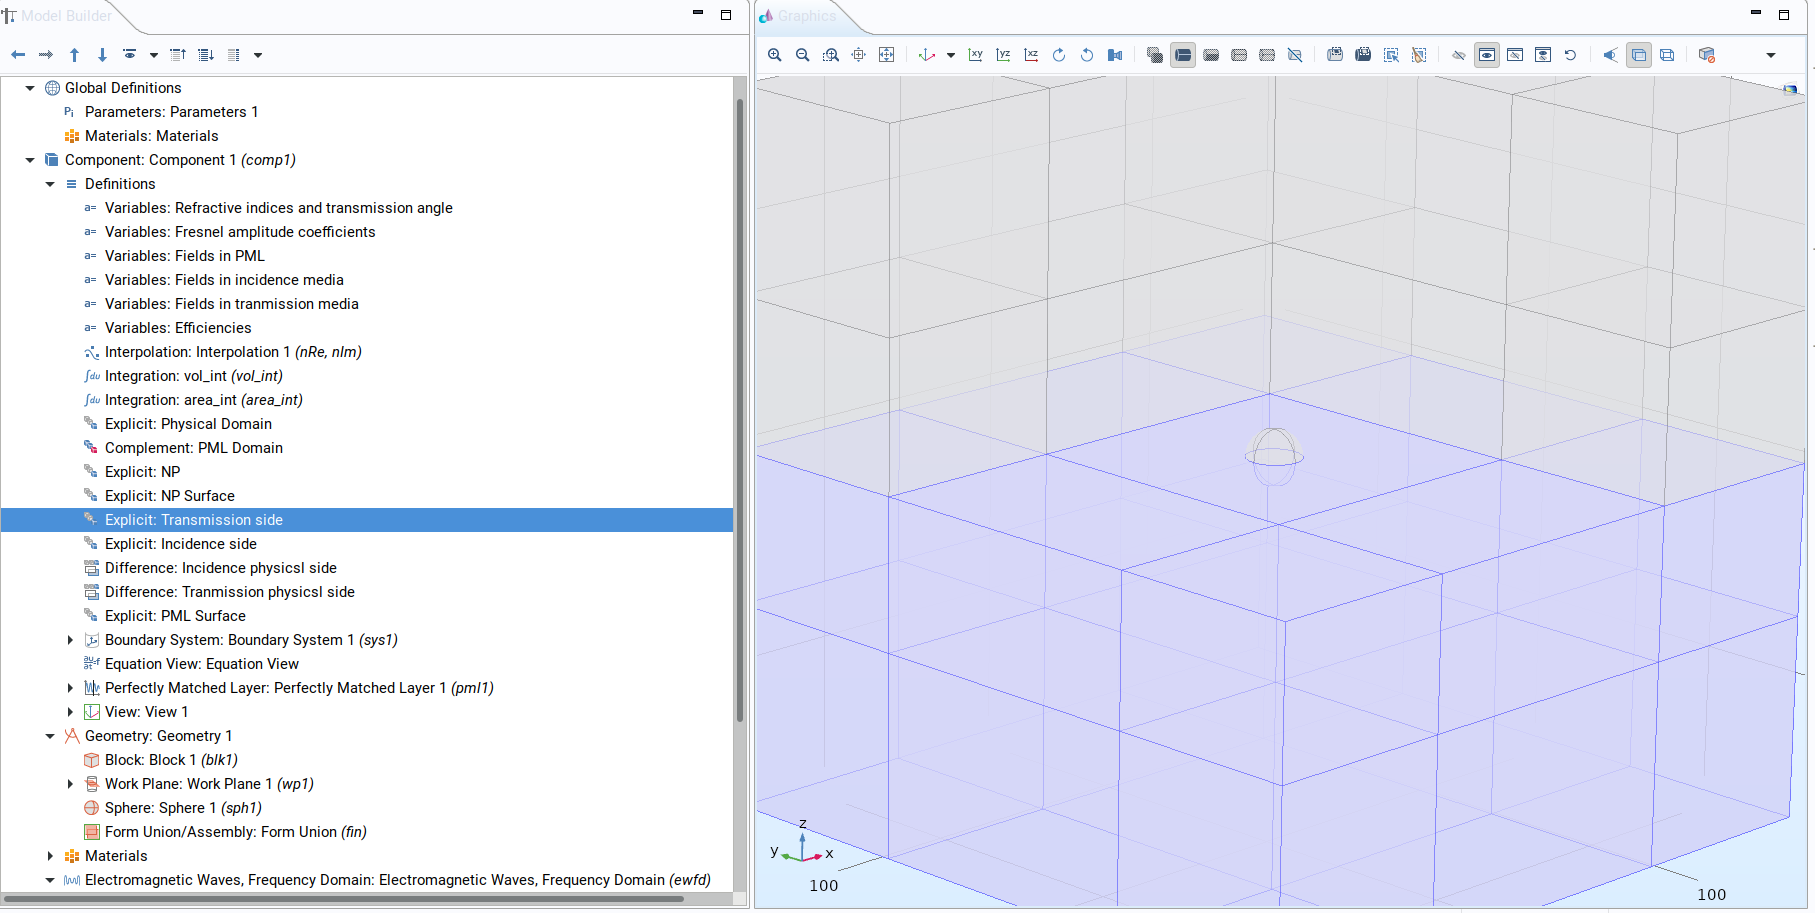
\includegraphics[width = .9 \textwidth]{COMSOL/Geometry.png}
\caption[COMSOl File Screenshot: Components/Definitions and Components/Geometry]{Screenshot of a COMSOL Multiphysics™ Ver. 5.4 file showing the Model Builder (left panel) and the Graphics of the built Geometry (right panel). In the Model Builder the Definitions and Geometry sections in Component are expanded to show their contents.}
\label{fig:COMSOL-Geo}
\end{figure}

With the made volume and surface definitions, integral operators can be defined. In particular, it can be seen in Fig. \ref{fig:COMSOL-Geo} that the volume integral operator of a scalar quantity is defined as \lstinline!vol_int!, where the integration volume is \lstinline!NP! and a surface integral operators in the surface \lstinline!NP Surface! is defined as \lstinline!area_int!. Besides integral operators, one can define functions from interpolation of data points, which is the case of the functions \lstinline!nRe! and \lstinline!nIm! that correspond to the real and the imaginary parts of the size corrected refractive index of a gold nanoparticle ---see Appendix \ref{app:SizeCorrection}---. The PML of the system requires to be set in the Component/Definitions section by choosing this option in its menu and applying it to the \lstinline!PML Domain! subvolume. Lastly, within Component/Definitions one can define local variables into a subvolume or for the whole system; this COMSOL's function was used to define the external electric field which corresponds to an incident, a reflected and a transmitted electric plane wave. These three contributions were defined piecewise in three subvolumes: \lstinline!Physical incidence side!, \lstinline!Physical transmission side! and \lstinline!PML Domain!. On the one hand, in Table \ref{tab:Incident-parameters} there are shown the phase of the incident and reflected electric fields, defined as \lstinline!k_i! and \lstinline!k_r!, respectively, as well as their three spatial components ---\lstinline!Ei_x!, \lstinline!Ei_y! and \lstinline!Ei_z! for the incident plane wave and \lstinline!Ert_x!, \lstinline!Ert_y! and \lstinline!Ert_z! for the reflected plane wave---, alongside the Fresnel's reflection amplitude coefficients for both \textit{s} (\lstinline!r_s!) and \textit{p} (\lstinline!r_p!) polarization. On the other hand, in Table \ref{tab:Transmission-parameters} the three spatial components ---\lstinline!Ert_x!, \lstinline!Ert_y! and \lstinline!Ert_z!--- and the phase ---\lstinline!k_t!--- of the transmitted electric field are defined, as well as Fresnel's transmission amplitude coefficients for both \textit{s} (\lstinline!t_s!) and \textit{p} (\lstinline!t_p!) polarization; the component of the incident electric field are all set equal to zero. Additionally, the external electric field is set to zero in the \lstinline!PML Domain!, as shown in Table \ref{tab:PML-parameters}.

Before defining the scattering, absorption and extinction cross sections in the Component/Definitions section, one must choose the PDE problem to be solved in the Electromagnetic Waves, Frequency Domain (\lstinline!ewfd!) and set its formulation in Scattered Field and choose the external electric field, defined piecewise in Tables \ref{tab:Incident-parameters}--\ref{tab:PML-parameters}, as the sum of the incident, the reflected and the transmitted plane waves. This can be done in the settings panel of \lstinline!ewfd! as shown in Fig. \ref{fig:COMSOL-Eq}, where the Scattering formulation allows the user to use the generalized Sommerfeld's  radiation condition [Eq. \eqref{eq:SommVec}] and to separate the contributions of the total electric field into the external and the induced electric fields, as well as to access to precomputed physical quantities related to the calculated electric field, such as the Poynting vector, for example.

\begin{sidewaystable}
 \caption{Local definitions for COMSOL simulation: Component/Definitions/Variables. The below variables are locally defined in the subvolume \lstinline!Physical incidence side!. }
 \label{tab:Incident-parameters}
    \centering
    \footnotesize
    \begin{tabular*}{.94\textwidth}{ |l|l|l| }
     \hline
     \textbf{Name}      &   \textbf{Expression}                                                                                 &   \textbf{Description} \\ \hline \hline
     \lstinline!k_ir!   &    \lstinline!(2*pi/wlength)*n_i*(x*sin(theta_i)*cos(phi)+y*sin(theta_i)*sin(phi)+z*cos(theta_i))!     &   Incident plane wave phase          \\
     \lstinline!k_rr!   &    \lstinline!(2*pi/wlength)*n_i*(x*sin(theta_i)*cos(phi)+y*sin(theta_i)*sin(phi)-z*cos(theta_i))!     &   Reflected plane wave phase         \\
     \lstinline!Ei_x!   &   \lstinline!(-E_s*sin(phi) - E_p*cos(theta_i)*cos(phi) ) * exp(-j*k_ir)!                              &   Incident plane wave - x component  \\
     \lstinline!Ei_y!   &   \lstinline!( E_s*cos(phi) + E_p*cos(theta_i)*sin(phi) ) * exp(-j*k_ir)!                              &   Incident plane wave - y component  \\
     \lstinline!Ei_z!   &   \lstinline! E_p*sin(theta_i) * exp(-j*k_i)!                                                         &   Incident  plane wave - z component \\
     \lstinline!r_s!    &   \lstinline!(n_i*cos(theta_i)-n_t*cos(theta_t))/(n_i*cos(theta_i)+n_t*cos(theta_t))!                 &   S reflection amplitude coefficient \\
     \lstinline!r_p!    &   \lstinline!(n_t*cos(theta_i)-n_i*cos(theta_t))/(n_t*cos(theta_i)+n_i*cos(theta_t))!                 &   P reflection amplitude coefficient \\
     \lstinline!Ert_x!  &   \lstinline!(-E_s*sin(phi)*r_s - E_p*cos(theta_i)*cos(phi)*r_p ) * exp(-j*k_rr)!                      &   Reflected plane wave - x component \\
     \lstinline!Ert_y!  &   \lstinline!( E_s*cos(phi)*r_s - E_p*cos(theta_i)*sin(phi)*r_p ) * exp(-j*k_rr)!                      &   Reflected plane wave - y component \\
     \lstinline!Ert_z!  &   \lstinline! E_p*sin(theta_i)*r_p * exp(-j*k_rr)!                                                     &   Reflected plane wave - z component \\
     \hline \hline
    \end{tabular*}
 \vspace*{1.5em}
 \caption{Local definitions for COMSOL simulation: Component/Definitions/Variables. The below variables are locally defined in the subvolume \lstinline!Physical transmission side!. }
 \label{tab:Transmission-parameters}
    \begin{tabular*}{.9606\textwidth}{ |l|l|l| }
     \hline
     \textbf{Name}          &   \textbf{Expression}                                                                                  &   \textbf{Description} \\ \hline \hline
     \lstinline!k_tr!        &   \lstinline!(2*pi/wlength)*n_t*(x*sin(theta_t)*cos(phi)+y*sin(theta_t)*sin(phi)+z*cos(theta_t))!      &   Transmitted plane wave phase         \\
     \lstinline!Ei_x!       &   \lstinline!0.!                                                                                       &   Incident plane wave - x component    \\
     \lstinline!Ei_y!       &   \lstinline!0.!                                                                                       &   Incident plane wave - y component    \\
     \lstinline!Ei_z!       &   \lstinline!0.!                                                                                       &   Incident plane wave - z component    \\
     \lstinline!t_s!        &   \lstinline!2*n_i*cos(theta_i)/(n_i*cos(theta_i)+n_t*cos(theta_t))!                                   &   S amplitude transmssion coefficient  \\
     \lstinline!t_p!        &   \lstinline!2*n_i*cos(theta_i)/(n_t*cos(theta_i)+n_i*cos(theta_t))!                                   &   P amplitude transmssion coefficient  \\
     \lstinline!Ert_x!      &   \lstinline!(-E_s*sin(phi)*t_s - E_p*cos(theta_t)*cos(phi)*t_p ) * exp(-j*k_tr)!                       &   Transmitted plane wave - x component \\
     \lstinline!Ert_y!      &   \lstinline!( E_s*cos(phi)*t_s - E_p*cos(theta_t)*sin(phi)*t_p ) * exp(-j*k_tr)!                       &   Transmitted plane wave - y component \\
     \lstinline!Ert_z!      &   \lstinline! E_p*sin(theta_i)*t_p * exp(-j*k_tr)!                                                      &   Transmitted plane wave - z component \\
     \hline \hline
    \end{tabular*}
 \vspace*{1.5em}
 \caption{Local definitions for COMSOL simulation: Component/Definitions/Variables. The below variables are locally defined in the subvolume  \lstinline!PML Domain!.  }
 \label{tab:PML-parameters}
     \begin{tabular*}{.501\textwidth}{ |l|l|l| }
     \hline
     \textbf{Name}          &   \textbf{Expression}              &   \textbf{Description} \\ \hline \hline
     \lstinline!Ei_x!       &   \lstinline!0.!                   &   Incident electric plane wave - x component \\
     \lstinline!Ei_y!       &   \lstinline!0.!                   &   Incident electric plane wave - y component \\
     \lstinline!Ei_z!       &   \lstinline!0.!                   &   Incident electric plane wave - z component \\
     \lstinline!Ert_x!      &   \lstinline!0.!                   &   (Reflected) Transmittedd plane wave - x component \\
     \lstinline!Ert_y!      &   \lstinline!0.!                   &   (Reflected) Transmitted plane wave - y component  \\
     \lstinline!Ert_z!      &   \lstinline!0.!                   &   (Reflected) Transmitted plane wave - z component \\
     \hline \hline
    \end{tabular*}
\end{sidewaystable}

\begin{figure}[h!]
    \centering
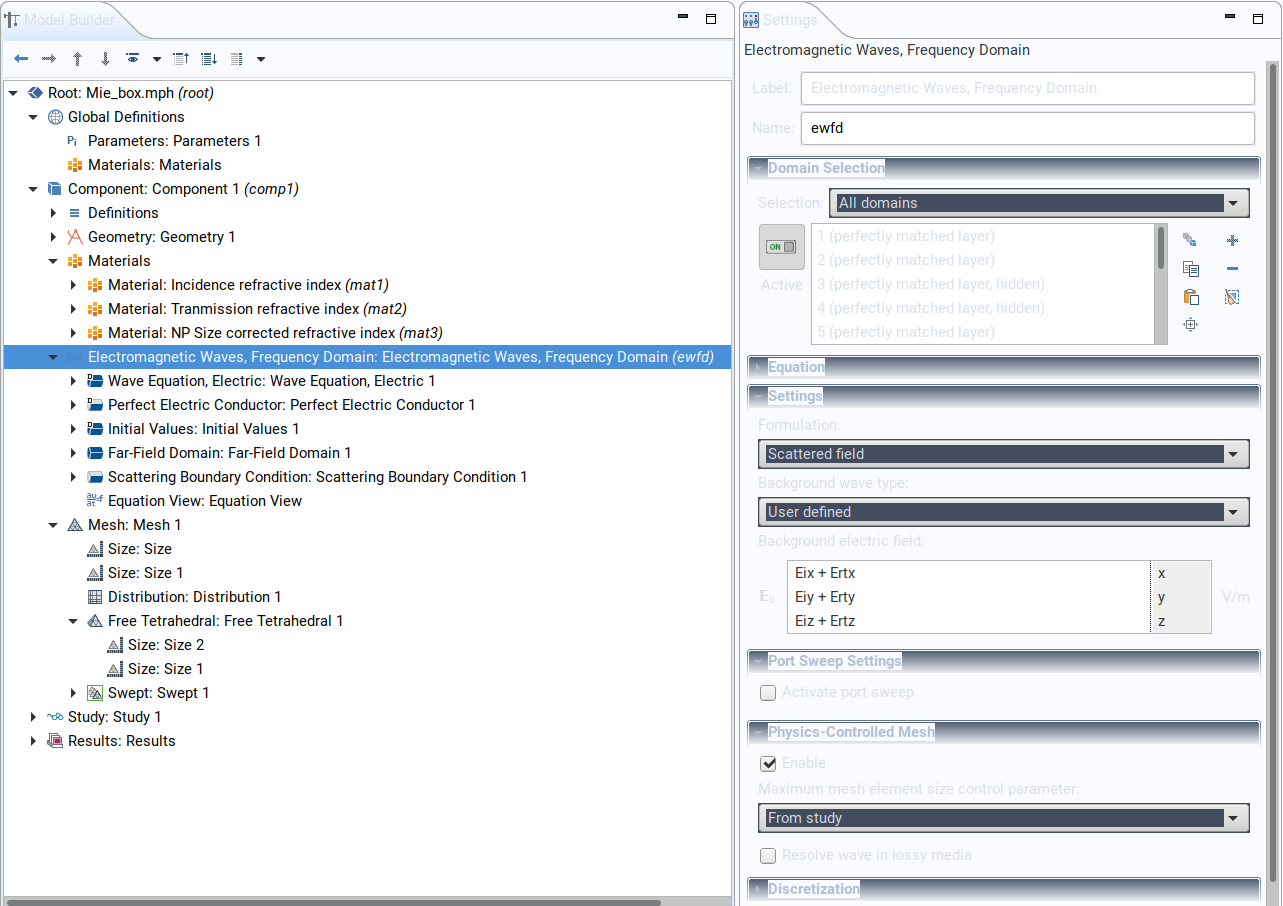
\includegraphics[width = .6 \textwidth]{COMSOL/Equation.png}
\caption[COMSOl File Screenshot: Components/Material and Components/ewfd]{Screenshot of a COMSOL Multiphysics™ Ver. 5.4 file showing the Model Builder (left panel) and the settings panel of the Electromagnetic Waves, Frequency Domain ---\lstinline!ewfd!--- (right panel). In the Model Builder the Materials and \lstinline!ewfd! sections in Components are expanded to show their content, while in the settings planel in \lstinline!ewfd! it is shown that the Scattered Field formulation is set and that the external electric field is a user-defined quantity given by the expressions shown in Tables \ref{tab:Incident-parameters}--\ref{tab:PML-parameters}.}
\label{fig:COMSOL-Eq}
\end{figure}


\begin{table}[b!]
\caption{Local definitions for COMSOL simulation: Component/Definitions/Variables. The below variables are locally defined in all domains. }
\label{tab:Domain-parameters}
\centering
\begin{tabular}{ |l|l|l| }
 \hline
 \textbf{Name}          &   \textbf{Expression}                         &    \textbf{Description} \\ \hline \hline
 \lstinline!theta_t!    &   \lstinline!arcsin((n_i/n_t)*sin(theta_i))!  &  Transmssion angle   \\
 \lstinline!S_i!        &   \lstinline!n_i*E0^2/(2*Z0_const)!           &    Incident Irradiance \\
 \lstinline!S_x!        &   \lstinline!nx * ewfd.relPoavx!              &    Average Poyting Vector in the normal x direction \\
 \lstinline!S_y!        &   \lstinline!ny * ewfd.relPoavy!              &    Average Poyting Vector in the normal y direction \\
 \lstinline!S_z!        &   \lstinline!nz * ewfd.relPoavz!              &    Average Poyting Vector in the normal z direction \\
 \lstinline!C_sca!      &   \lstinline!area_int(S_x + S_y + S_z)/(S_i)! &   Scattering cross section \\
 \lstinline!C_abs!      &   \lstinline!vol_int(ewfd.Qh)/(S_i)!          &   Absorption cross section \\
 \lstinline!C_ext!       &  \lstinline!C_sca + C_abs!                 &   Extinction cross section \\
 \hline \hline
\end{tabular}
\end{table}

After the Scattering Formulation of the \lstinline!ewfd! is set, and the external electric field was introduced into COMSOL's interface, the scattering, absorption and extinction cross sections are defined in the Component/Definitions section as a variable in the whole system. Since the scattering cross section is calculated by Eq. \eqref{eq:Csca}, the time-averaged scattering Poynting vector is projected onto the normal vector to a closed surface and then integrated on such surface. The component of the time-averaged scattering Poynting vector are precalculated by COMSOL and are accessed by the user thought the variables  \lstinline!ewfd.relPoavx!, \lstinline!ewfd.relPoavy! and \lstinline!ewfd.relPoavz! \cite{comsol_wave} and the component of the normal vector to any surface are given by \lstinline!nx!, \lstinline!ny! and \lstinline!nz!. By calculating the dot product of the normal vector and the time-averaged scattering Poynting vector, applying to it the integral operator \lstinline!area_int! and dividing by the irradiance of the incident plane wave \lstinline!S_i!, the scattering cross section  \lstinline!C_sca! is obtained. For the absorption cross section \lstinline!C_abs! the Eq. \eqref{eq:Cabs} is employed, that is the integral operator \lstinline!vol_int! is applied to the variable \lstinline!ewfd.Qh!, which are the heat losses calculated by Joule's law \cite{comsol_wave}; lastly the extinction cross section \lstinline!C_ext! is calculated as the sum of the scattering and the absorption cross sections. All the needed definitions are shown in Table \ref{tab:Domain-parameters}.

The last step before running the FEM simulation in COMSOL is to define the mesh ---or the partition into finite elements--- of the system.  As discussed in Section \ref{sec:FEM-Mie}, the mesh size can be set for different subvolumes in the system, as also the geometric shape of the finite elements. For this work tetrahedral finite element were chosen for the meshing in the matrix and the spherical scatterer (blue regions in Fig. \ref{fig:COMSOL-Mesh}), where the later had a finer meshing to diminish the absolute error of the obtained approximated solution. This is specified in the Component/Mesh section of the Model Builder by setting two different sizes to each subvolume of interest. Since the PML requires a geometrical transformation to simulate an absorbing media with no reflection, the finite elements in the PML must match the  geometrical symmetry of the system to minimize errors \cite{comsol_doc}, which is a rectangular or Cartesian symmetry in the employed geometry, as seen in the gray areas of  Fig. \ref{fig:COMSOL-Mesh}. Following the described steps in this section, the  geometry and boundary conditions employed in this work can be reproduced. After the system is set up, one can choose any Study and visualize the results in COMSOL's viewer or export them.

\begin{figure}[h!]
    \centering
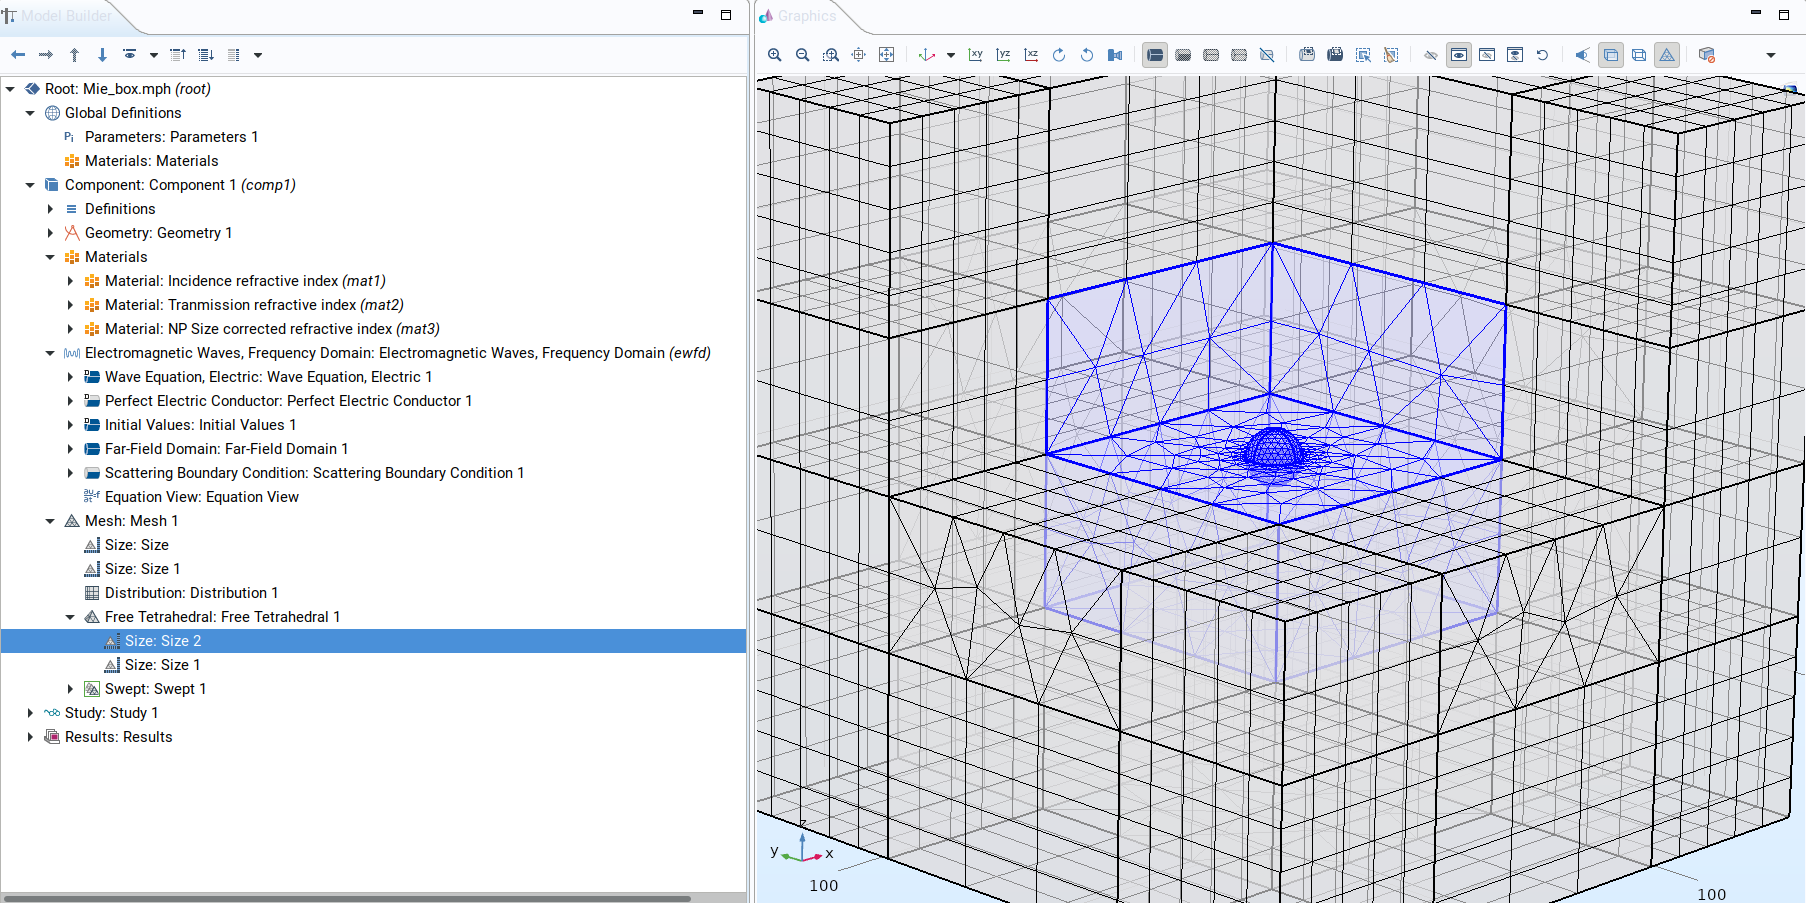
\includegraphics[width = .9 \textwidth]{COMSOL/Mesh.png}
\caption[COMSOl File Screenshot: Component/Materials, Component/ewfd and Component/Mesh]{Screenshot of a COMSOL Multiphysics™ Ver. 5.4 file showing the Model Builder (left panel) and the Graphics of the built geometry with the chosen mesh (right panel). In the Model Builder the Materials, Electromagnetic Waves, Frequency Domain ---\lstinline!ewfd!--- and Mesh sections in Component are expanded to show their contents.}
\label{fig:COMSOL-Mesh}
\end{figure}
